\documentclass[12pt]{article}
\usepackage{graphicx, color}
\usepackage[utf8]{inputenc}
\usepackage{amsfonts}
\usepackage{amsmath}
\usepackage[T1]{fontenc}
\usepackage{xcolor}
\usepackage{float}
\usepackage{textcomp}
\usepackage{multicol}
\usepackage[portuges]{babel}
\usepackage{xcolor}
\usepackage[round]{natbib}
\usepackage[utf8]{inputenc}
\usepackage{amsmath,amssymb}
\usepackage{hyperref}
\usepackage{longtable}
\usepackage{subfig}
\usepackage{soul}

\vfuzz2pt
\hfuzz2pt
\newtheorem{thm}{Theorem}[section]
\newtheorem{cor}[thm]{Corollary}
\newtheorem{lem}[thm]{Lemma}
\newtheorem{prop}[thm]{Proposition}
\newtheorem{defn}[thm]{Definition}
\newtheorem{rem}[thm]{Remark}
\numberwithin{equation}{section}
\newcommand{\norm}[1]{\left\Vert#1\right\Vert}
\newcommand{\abs}[1]{\left\vert#1\right\vert}
\newcommand{\set}[1]{\left\{#1\right\}}
\newcommand{\Real}{\mathbb R}
\newcommand{\eps}{\varepsilon}
\newcommand{\To}{\longrightarrow}
\newcommand{\BX}{\mathbf{B}(X)}
\newcommand{\A}{\mathcal{A}}
\usepackage{anysize}
\usepackage[left=2.0cm,top=2.5cm,right=1.5cm,bottom=2.0cm]{geometry} 




\renewcommand*\contentsname{Conteúdo}

%\title{}
%\date{}
\begin{document}
\thispagestyle{empty} 


%%%%%%%%%%%%%%%%%%%%%%%%%%%%%%%%%%%%%%%%%%%%%%%%%%%%%%%%%%%%%%%%%%%%%%%%%%%%%%%%%%%%%%%%%
%%%%%%% 			CAPA DO TRABALHO ou Folha de rosto					 	 %%%%%%%%%%%%
%a. Folha de rosto, contendo os seguintes itens:							
%• Nome do aluno;
%• Nome do orientador e coorientador, se houver;
%• Data de início do Doutorado;
%• Se for bolsista, nome da agência financiadora e data de início da bolsa;
%%%%%%%%%%%%%%%%%%%%%%%%%%%%%%%%%%%%%%%%%%%%%%%%%%%%%%%%%%%%%%%%%%%%%%%%%%%%%%%%%%%%%


\begin{figure}
  \centering
  
\includegraphics[scale=0.5]{logoon.png}
  \vspace*{-0.3cm}
\end{figure}

\begin{center}
{\large \rm \textbf {OBSERVATÓRIO NACIONAL} \linebreak}
{\large \rm \textbf {MINISTÉRIO DA CIÊNCIA E TECNOLOGIA} \linebreak}
{\large \rm \textbf {PROGRAMA DE PÓS-GRADUAÇÃO EM ASTRONOMIA} \linebreak}
\end{center}

\baselineskip 30pt

\vspace*{0.3cm}

\begin{center}
{\LARGE \bfseries Relatório de Atividades }
\end{center}

\vspace*{1cm}

\setcounter{footnote}{1}

\renewcommand{\thefootnote}{\fnsymbol{footnote}}
\begin{center}
{\sc  Aluno: Thiago Laidler Vidal Cunha

\vspace*{0.3cm}

{\sc  Orientador: Julio Ignacio Bueno de Camargo
\\}

\end{center}

\setcounter{footnote}{1}

\vspace*{2.8cm}

\begin{flushleft}
Início do Mestrado: Março de 2024\\
Bolsa: Sem bolsa\\
\end{flushleft}


\baselineskip 17pt

\vspace*{1.5cm}
\begin{center}
{{\bf Rio de Janeiro\par{Agosto de 2025}}}
\end{center}

\vspace*{.05cm}


\renewcommand{\thefootnote}{\arabic{footnote}}

\setcounter{footnote}{1}

\pagebreak

\baselineskip 19pt

%%%%%%%%%%%%%%%%%%%%%%%%%%%%%%%%%   CAPITULO 1 %%%%%%%%%%%%%%%%%%%%%%%%%%%%%%%%%%%%%%%%%%%%%%%%%


\pagenumbering{roman}
\pagestyle{fancy}
\tableofcontents
\pagenumbering{arabic}


%*****************************************************************
%PROJETO
%*****************************************************************

\newpage

\section{\sc Projeto}

O projeto de mestrado intitulado "Pipeline para Detecção Automatizada de Ocultações Estelares em Curvas de Luz com Técnicas de Machine Learning" propõe uma abordagem nova para um dos desafios emergentes da astronomia moderna: o tratamento do crescente volume de dados de observações de ocultações estelares. Essas ocultações - eventos em que um corpo celeste, como um asteroide, passa em frente a uma estrela e bloqueia sua luz - são ferramentas poderosas para a caracterização física e orbital desses corpos. No entanto, a análise manual das curvas de luz resultantes é cada vez mais difícil, dada a grande quantidade e complexidade dos dados.

O principal objetivo do projeto é desenvolver um modelo automatizado baseado em técnicas de machine learning, capaz de identificar, em grandes conjuntos de curvas de luz, sinais da existência de ocultação estelar. Mais do que apenas classificar como “ocultação” ou “não ocultação”, o sistema pretende também auxiliar na análise de eventos cujas quedas de brilho estejam muito próximas do nível de ruído e que, por isso, necessitem de investigação mais detalhada ou de observações adicionais para eventual confirmação. Essa abordagem tem o potencial de otimizar bastante o tempo dos pesquisadores para tais casos limítrofes, além de também permitir o escalonamento das análises para volumes de dados que seriam inviáveis por métodos tradicionais.

A primeira fase do projeto concentrou-se na engenharia de dados, etapa essencial para a aplicação de modelos de aprendizado de máquina. Foram compiladas curvas de luz provenientes de diversas fontes e integradas em um banco de dados relacional SQL. Para facilitar a organização e o acesso a esses dados, foram desenvolvidos scripts de consulta e pré-processamento, permitindo a geração de datasets treináveis com diferentes recortes e características.

Devido à escassez de eventos positivos de ocultações reais disponíveis para treinamento, será necessário empregar técnicas de geração sintética de dados - baseado na metodologia de \cite{Simulator}. Essas curvas artificiais serão construídas com base em parâmetros físicos do corpo ocultador (tamanho, composição), tempo de observação e localização do observador. Também será aplicada a técnica de \textit{data augmentation}, utilizando recortes de curvas positivas reais (em trechos onde nitidamente não continham eventos) para equilibrar a proporção entre eventos positivos e negativos na base de dados. 

Além disso, cada curva será enriquecida com atributos estatísticos, como média, desvio padrão, fluxo mínimo e máximo, e as médias dos fluxos em cada quartil. Esses parâmetros servem para auxiliar no treinamento de modelos supervisionados, fornecendo insumos relevantes para a diferenciação entre eventos reais e falsos positivos. Mais parâmetros estão sendo estudados para serem adicionados no dataset.

Atualmente, o projeto se encontra na etapa de rebalanceamento do dataset para imediato treinamento e comparação entre modelos de \textit{machine learning}, com foco nos algoritmos XGBoost e \textit{Random Forest}. Ambos são amplamente reconhecidos por sua robustez em tarefas de classificação, especialmente em contextos com dados tabulares e variabilidade significativa entre instâncias. A escolha desses modelos se justifica por sua capacidade de generalização e pela interpretabilidade das variáveis mais relevantes para a predição.

Futuramente, pretende-se também explorar redes neurais convolucionais (\textit{CNNs}), dado seu sucesso prévio em aplicações similares, como no modelo \textit{ODNet}, utilizado pela \textit{Unistellar Network} \cite{Cazeneuve_2023}, que alcançou 91\% de acurácia e 87\% de \textit{recall}, com capacidade de processar múltiplas curvas por segundo. %citar Cazeneuve_2023


\subsection{Objetivo Científico}
\indent
O projeto possui dois objetivos principais:

\begin{itemize}
    \item Organizar e disponibilizar um banco de curvas de luz estruturado, servindo como recurso para futuras pesquisas em ocultações estelares;
    \item Desenvolver uma ferramenta automatizada de classificação, capaz de identificar rapidamente quais curvas apresentam ocultações reais, auxiliando astrônomos na triagem e análise dos dados.
\end{itemize}

Além de acelerar significativamente o processo de análise, o modelo também poderá detectar eventos sutis ou de difícil interpretação, fornecendo uma estimativa probabilística da ocorrência de uma ocultação. Esse aspecto é particularmente importante diante das limitações de ferramentas legadas, que frequentemente geram falsos positivos, especialmente em observações de estrelas de brilho mais tênue.

Com o avanço do pipeline, espera-se pavimentar o caminho para sistemas de detecção autônoma de eventos raros, como ocultações por objetos transnetunianos ou asteroides ainda não catalogados - ampliando assim a capacidade de descoberta da astronomia observacional.

\subsection{Metodologia a ser Utilizada}
\indent
A metodologia deste projeto teve início com uma fase rigorosa de engenharia de dados, que envolveu a coleta, padronização e consolidação de curvas de luz provenientes de diferentes fontes em um banco de dados relacional estruturado em SQL. 

Historicamente, os dados de observações de ocultações estelares não eram de fácil acesso, sendo frequentemente necessário entrar em contato individualmente com astrônomos ou grupos de pesquisa para obtê-los. Embora o número de registros tenha crescido nos últimos anos, a quantidade disponível ainda é relativamente limitada, o que dificulta a formação de um conjunto de dados extenso para aplicações de aprendizado de máquina. Além disso, as poucas bases públicas existentes concentram-se majoritariamente em curvas de rotação de corpos menores (o que não agrega ao escopo do projeto) ou curvas positivas (com detecção de evento), o que não contempla um número expressivo de curvas negativas. Diante desse cenário, adotaremos uma estratégia de balanceamento do conjunto de dados, que inclui a ampliação da classe negativa por meio do recorte de trechos de curvas reais sem eventos e a geração de curvas sintéticas simuladas com base em parâmetros físicos como tamanho do corpo ocultador, composição, duração da observação e localização geográfica do observador. Essas simulações são fundamentais para enriquecer o conjunto de treinamento e permitir a generalização dos modelos. Posteriormente, cada curva de luz será transformada em uma representação vetorial por meio da extração de estatísticas descritivas relevantes, como média, desvio padrão, valores mínimo e máximo do fluxo, além de médias condicionais em cada quartil.

Esses atributos funcionarão como medidas-resumo capazes de capturar padrões importantes no comportamento das curvas, tornando-as adequadas para serem interpretadas por algoritmos de aprendizado de máquina. 

Por fim, iremos comparar diferentes modelos para decidir qual o mais preciso e acurado.

\subsection{Resultados Esperados}
\indent
Com base na metodologia proposta, espera-se que os algoritmos de machine learning empregados - em especial os modelos de XGBoost e Random Forest - apresentem elevado desempenho na classificação de curvas, diferenciando com precisão eventos com e sem ocultações. Esperamos detecção de ocultações em casos complicados, com curvas de luz de alto ruído e ocultações curtas. A meta é atingir resultados comparáveis ou superiores aos obtidos por redes neurais convolucionais, que já demonstraram acurácia de 91\% e recall de 87\% em tarefas semelhantes - \cite{Cazeneuve_2023}, beneficiando-se aqui de um processo rigoroso de engenharia de dados, otimização de hiperparâmetros e validação cruzada. 

Além disso, espera-se que este trabalho produza um banco de dados altamente estruturado de curvas de luz, promovendo padronização e facilitando o acesso e a análise por parte da comunidade astronômica. O modelo também deverá permitir a categorização automática de grandes volumes de dados, reduzindo a necessidade de inspeção manual e o risco de erro humano, além de fornecer estimativas probabilísticas em casos ambíguos, auxiliando na interpretação de eventos limítrofes.

\section{\sc Informações curriculares}


\subsection{Disciplinas Cursadas}

{\small
\begin{tabular}{|c|l|c|c|}
\hline
Ano/Semestre & Disciplina & Conceito & Créditos \\
\hline
2024/1       & Astronomia de Posição    & A & 4  \\
2024/1       & Evolução Estelar	& A & 4  \\
2024/2       & Astroestatística         & A & 4  \\
2024/1       & Astronomia Dinâmica      & A & 4  \\
2024/2       & Tópicos de E-Science     & A & 4  \\
2024/2       & Propriedades Físicas de Pequenos Corpos & A & 4 \\

\hline
\hline
\end{tabular}
}


\subsection{Atividades}

%%Jonatã:
%\begin{itemize}

%\item Apresentação de trabalho intitulado 'Determinação das curvas astrométricas de %\textit{precision premium} nos telescópios do Observatório do Pico dos Dias' na XLVI Reunião da %Sociedade Astronômica Brasileira de 2023, realizada entre 2 e 5 de outubro de 2023 no Rio de Janeiro;

%\item Participação do 'Workshop SPANet de Instrumentação Astronômica' realizado nos dias 16 e 17 de %novembro de 2023 (remoto);

%\item Participação no 'XII Taller de Ciencias Planetárias' realizado de 26 de fevereiro a 1° de %março de 2024 no Observatório Nacional, no Rio de Janeiro.

%\end{itemize}

% \subsection{Participação em publicações}
% (não sei se vale de alguma coisa colocar isso ...)
% {\sc Publicados}
% \begin{itemize}
%     \item Catani, L.M., Assafin, M., Morgado, B.E., Santos-Filho, S., Braga-Ribas, F., Vieira-Martins, R., \textbf{Arcas-Silva, J.}, Milone, A.C., Lima, I.J. and Botelho, R.B., 2023. The 2021 mutual phenomena involving the Galilean satellites of Jupiter and the inner satellite Thebe. Monthly Notices of the Royal Astronomical Society, 526(4), pp.6145-6154.
% \end{itemize}





%\subsection{ Publicações}

%{\sc Submetidos}

\subsection{Exame de Proficiência}

Aprovado no exame de proficiência oferecido pelo Observatório Nacional em 2024.


%%%%%%%%%%%%%%%%%%%%%%%%%%%%%%%%%%%%%%%%%%%%%%%%%%%%%%%%%%%%%%%%%%%%%%%%%%%%%%%%%%%%%
%%%%%%% 		Capitulo 3 |  principais avancos em relacao ao ultimo relatorio %%%%%
%d. Situação do projeto de pesquisa à época do último relatório;
%–no mínimo 1 (uma) e no máximo 2 (duas) páginas–;
%%%%%%%%%%%%%%%%%%%%%%%%%%%%%%%%%%%%%%%%%%%%%%%%%%%%%%%%%%%%%%%%%%%%%%%%%%%%%%%%%%%%%


\section{Situação do projeto à época do último relatório}

Esse é o primeiro relatório apresentado.


%%%%%%%%%%%%%%%%%%%%%%%%%%%%%%%%%   CAPITULO 4 %%%%%%%%%%%%%%%%%%%%%%%%%%%%%%%%%%%%%%%%%%%%%%%%%

\section{\sc Descrição detalhada da pesquisa}

\subsection{Metodologia Aplicada}\label{sec_met}
\indent
O trabalho teve início com a etapa de preparação e organização dos dados, na qual curvas de luz oriundas de múltiplas fontes foram padronizadas e integradas a um banco de dados relacional implementado em SQLite. Parte desse conjunto foi obtida a partir do banco de dados em nuvem do Grupo do Rio, referentes às ocultações por Umbriel - observadas em 2020, analisadas por \cite{Umbriel2020} - e Chiron - observadas em 2023 e analisadas por \cite{Chiron2023}. A maior parte dos dados, contudo, foi adquirida no portal VizieR, totalizando 931 curvas de luz em formato \texttt{.dat}, contendo séries temporais de fluxo de luz. Para cada curva, foram extraídas e armazenadas no banco as seguintes informações: série temporal da curva de luz, nome do objeto ocultador, data da observação, fonte dos dados, nome do observador e classificação do evento (ocultação positiva ou não). O processamento e integração dos dados foram realizados com auxílio das bibliotecas \texttt{Astropy} e \texttt{Astroquery} (leitura e consulta de arquivos astronômicos), \texttt{SQLAlchemy} (interface com o banco de dados), \texttt{asyncio} e \texttt{aiohttp} (coleta assíncrona), e \texttt{Pandas} (manipulação tabular).

Para possibilitar a integração eficiente dos dados coletados, foram desenvolvidos scripts em Python com funções específicas de consulta e organização, garantindo consistência e qualidade no armazenamento das informações. A primeira rotina, implementada de forma assíncrona, foi responsável por buscar e baixar o maior número possível de curvas de luz disponíveis no portal VizieR, reduzindo significativamente o tempo de aquisição dos dados. A segunda rotina teve como objetivo estruturar e compactar essas curvas em um banco de dados relacional no formato SQLite (\texttt{.db}), o que viabiliza consultas rápidas e organizadas.

   \begin{figure}[!h]
\begin{center}
	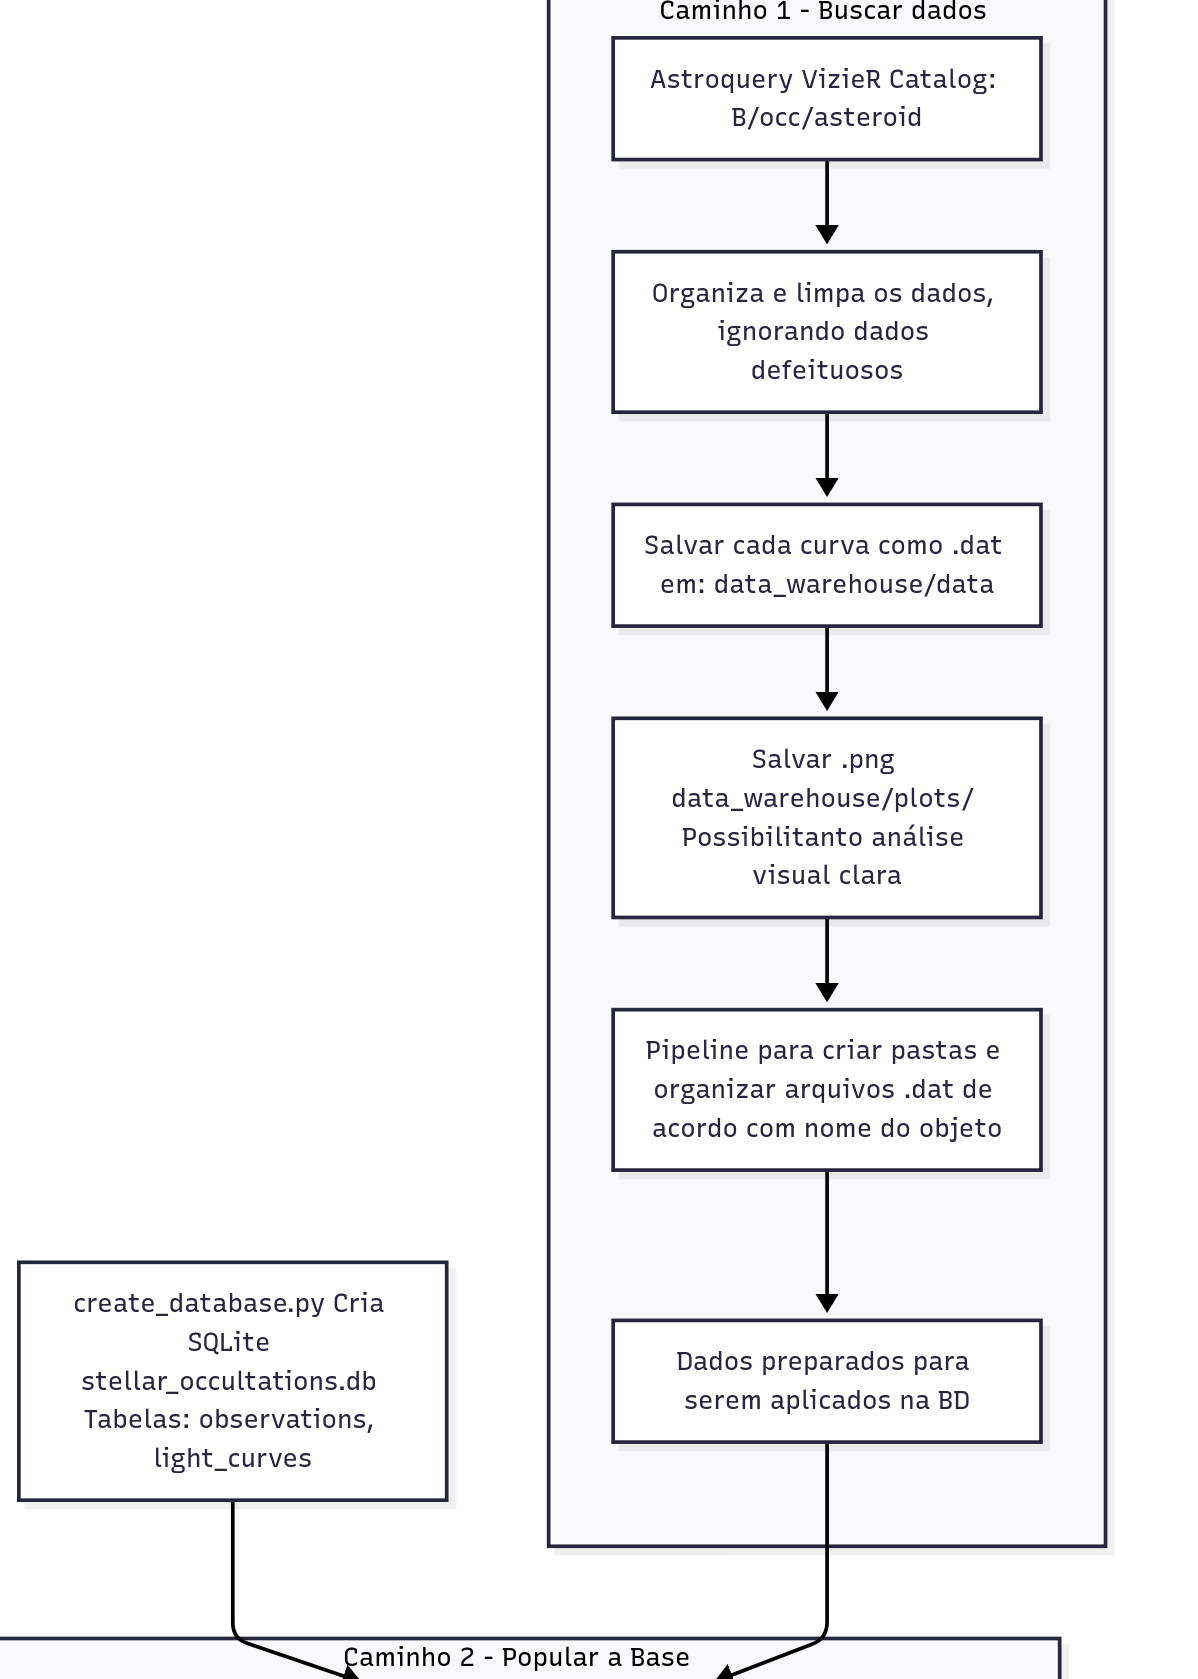
\includegraphics[scale=0.3]{fluxo1.png}
\caption{Fluxograma ilustrando o funcionamento dos scripts responsáveis pela aquisição e organização dos dados externos, bem como a integração desses dados na etapa subsequente de inserção no banco de dados SQL.}
\label{Fig1.1}
\end{center}
\end{figure}

O banco foi estruturado em duas tabelas principais: \texttt{observations}, que armazena informações gerais da observação (como nome do objeto, data, fonte dos dados e metadados adicionais), e \texttt{light curves}, que contém os pontos individuais da curva de luz (tempo e fluxo) vinculados à observação correspondente por meio de uma chave estrangeira (\texttt{observation id}). Essa arquitetura relacional foi concebida para manter a integridade referencial, preservar os dados originais e, ao mesmo tempo, facilitar consultas e análises posteriores.

Durante o processo de inserção no banco, buscou-se preservar ao máximo os valores observados, realizando apenas verificações e ajustes mínimos para garantir a consistência do registro. Esses ajustes incluíram a uniformização de formatos de unidades quando necessário, a checagem do alinhamento temporal informado e a validação de metadados, sem qualquer manipulação que alterasse as características intrínsecas das curvas. O uso de um formato relacional, aliado à automação das etapas de coleta e organização, assegura que o conjunto final esteja pronto para ser processado por modelos de aprendizado de máquina, mantendo a fidelidade aos dados originais e minimizando riscos de redundância ou distorção.

   \begin{figure}[!h]
\begin{center}
	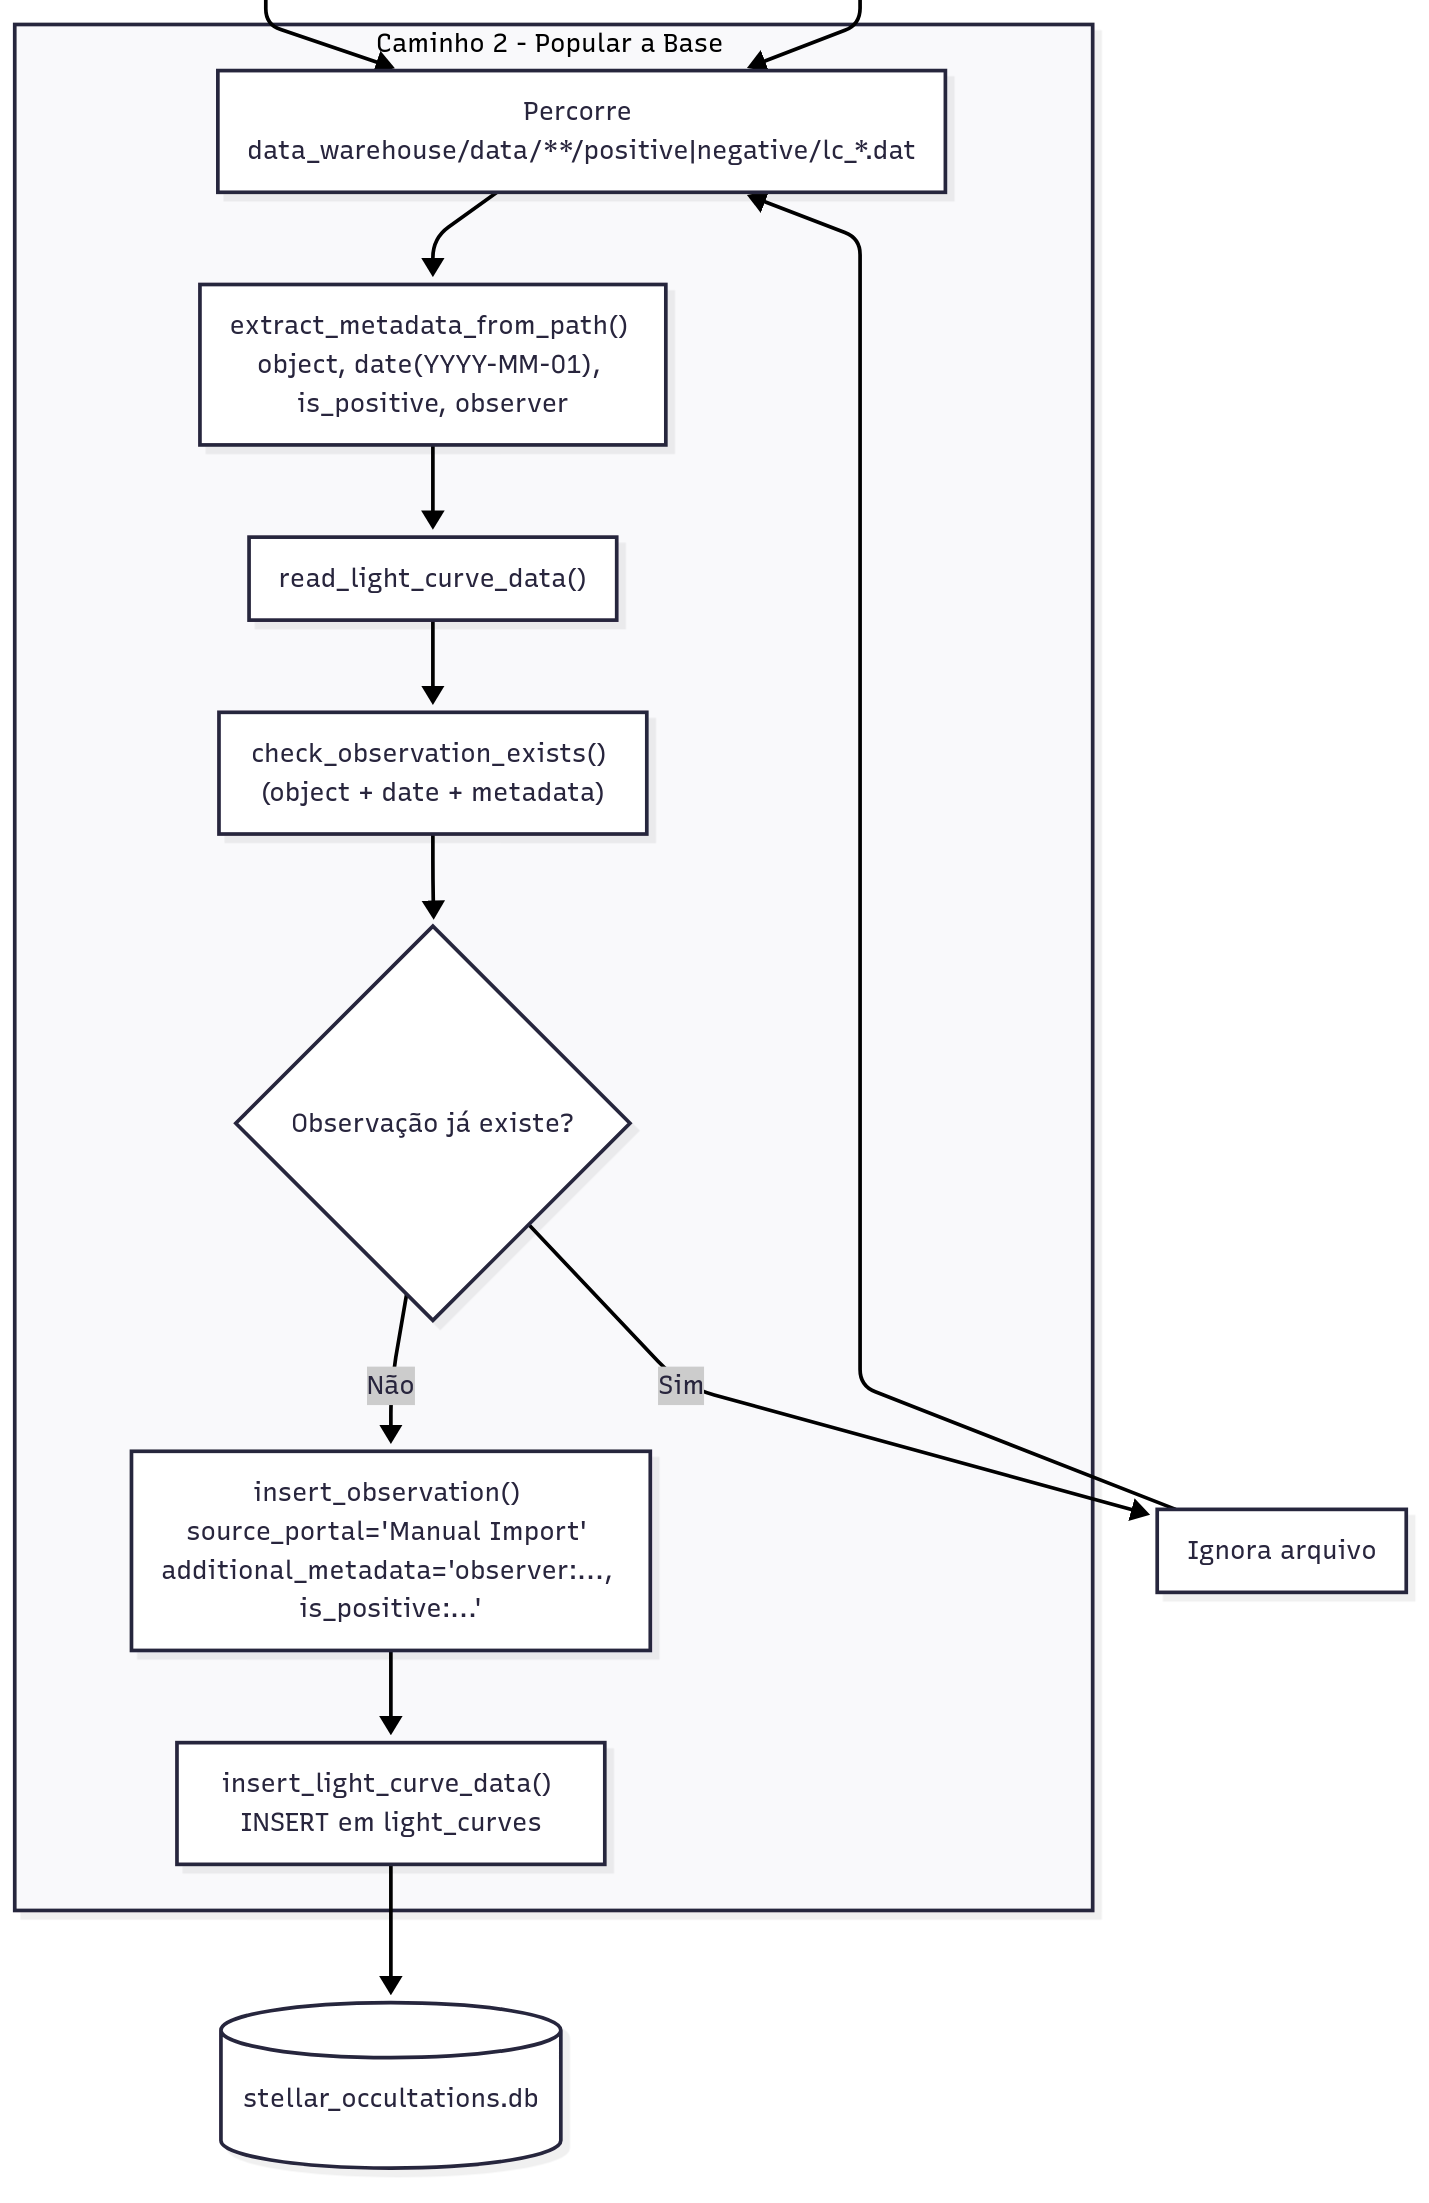
\includegraphics[scale=0.3]{fluxo2.png}
\caption{Fluxograma ilustrando a pipeline resonsável pela consolidação do Banco de Dados.}
\label{Fig1.2}
\end{center}
\end{figure}

Durante a aplicação da técnica de \textit{data augmentation} para ampliar a classe negativa, optou-se por realizar o recorte manual de segmentos de curvas de luz sem sinais de ocultação. Essa abordagem assegura que as amostras adicionadas ao conjunto de dados pertençam de fato à classe negativa, reduzindo o risco de viés que poderia ser introduzido por um processo automatizado com um modelo preliminar. Embora mais lenta e trabalhosa, essa estratégia contribui para a confiabilidade do conjunto de treinamento.

Está prevista a inclusão de curvas sintéticas negativas, visando diversificar os padrões presentes na classe negativa e aprimorar a capacidade de generalização do modelo final. Essas simulações são essenciais para enriquecer o conjunto de treinamento e aumentar a robustez do desempenho do modelo em diferentes condições observacionais.


   \begin{figure}[!h]
\begin{center}
	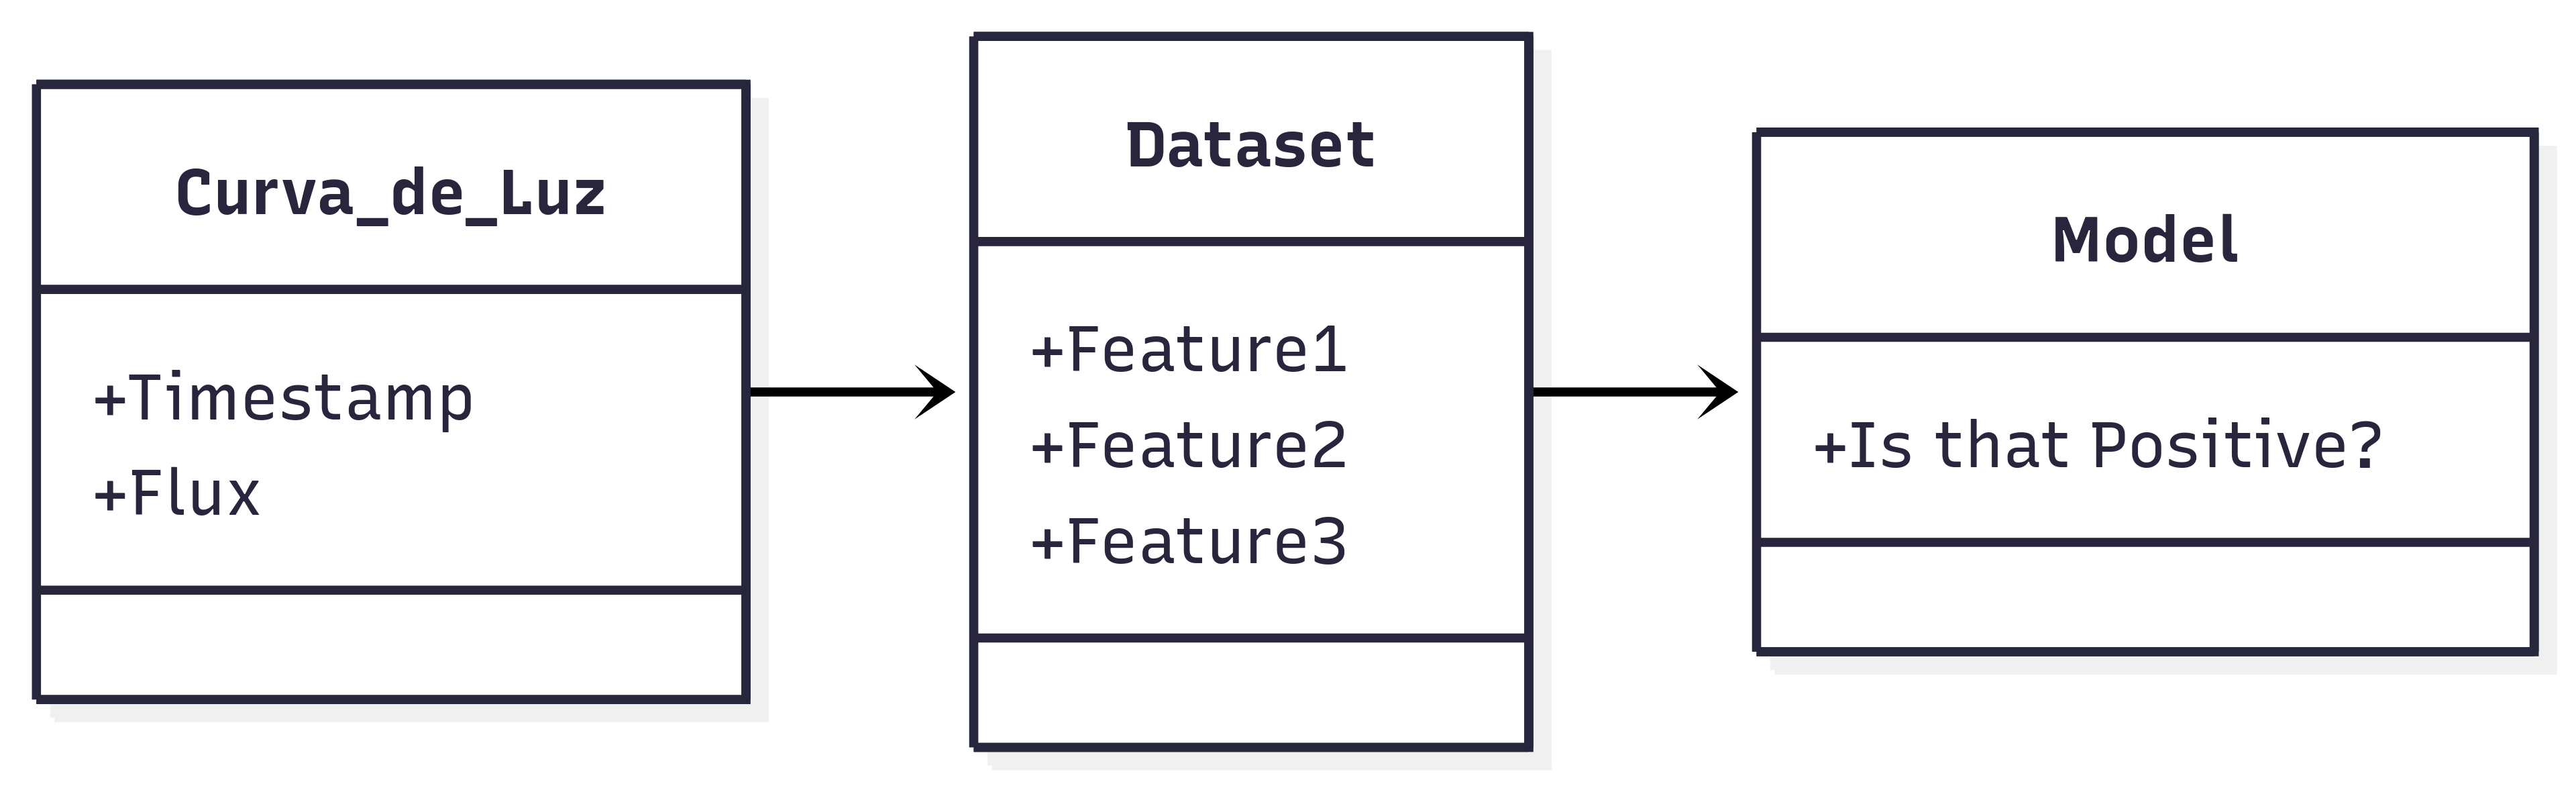
\includegraphics[scale=0.08]{Modelo.png}
\caption{Esquema do planejamento para o treinamento do modelo, destacando que serão utilizadas as características extraídas das curvas, e não as curvas originais em si.}
\label{Fig1.2}
\end{center}
\end{figure}

Em seguida, cada curva de luz será convertida em uma representação vetorial por meio da extração de estatísticas descritivas relevantes, tais como a média, o desvio padrão, os valores mínimo e máximo do fluxo, além de médias condicionais calculadas em cada quartil da série temporal. Outras possíveis características (\textit{features}) ainda estão sendo investigadas, com o objetivo de enriquecer o conjunto de atributos e aumentar a capacidade preditiva dos modelos.

Esses atributos funcionam como medidas-resumo que capturam padrões importantes no comportamento das curvas de luz, tornando-os adequados para serem interpretados por algoritmos de aprendizado de máquina.

A seguir, apresentamos as definições matemáticas das principais estatísticas que serão extraídas das curvas \(F(t)\), com \(N\) pontos de observação:

\[
\mu = \frac{1}{N} \sum_{i=1}^{N} F(t_i)
\]

\[
\sigma = \sqrt{\frac{1}{N - 1} \sum_{i=1}^{N} \left( F(t_i) - \mu \right)^2 }
\]

\[
F_{\min} = \min_{1 \leq i \leq N} F(t_i), \quad
F_{\max} = \max_{1 \leq i \leq N} F(t_i)
\]

Para a avaliação dos modelos de classificação binária, utilizaremos métricas consagradas como:

\textbf{Acurácia}:
\[
\text{Acurácia} = \frac{TP + TN}{TP + TN + FP + FN}
\]

\textbf{Precisão}:
\[
\text{Precisão} = \frac{TP}{TP + FP}
\]

\textbf{Recall} (Sensibilidade):
\[
\text{Recall} = \frac{TP}{TP + FN}
\]

\textbf{F1-score}:
\[
F_1 = 2 \times \frac{\text{Precisão} \times \text{Recall}}{\text{Precisão} + \text{Recall}}
\]

onde \(TP\), \(TN\), \(FP\) e \(FN\) representam, respectivamente, verdadeiros positivos, verdadeiros negativos, falsos positivos e falsos negativos.

Além dessas, será considerada a \textit{Área sob a Curva ROC} (AUC), que quantifica a capacidade do modelo em discriminar corretamente entre as classes positiva e negativa. Segundo o "Google Developers Machine Learning Course", a AUC representa "a probabilidade de que o modelo, quando confrontado com um exemplo positivo e outro negativo escolhidos ao acaso, atribua uma pontuação maior ao positivo do que ao negativo". Mais detalhes podem ser vistos em \cite{AUC-curve}, abordando fortalezas e fraquezas desse método.

Os modelos escolhidos para experimentação inicial são XGBoost e Random Forest, amplamente reconhecidos por seu desempenho em tarefas de classificação com dados tabulares. No entanto, outras abordagens poderão ser exploradas conforme o desenvolvimento do projeto.


% Incluir quais algoritmos foram testados (mesmo que o foco seja apenas em um)
% Descrever como o dataset foi dividido (treino/validação/teste) e se houve cross-validation
% Indicar métricas de avaliação planejadas (acurácia, F1-score, recall, etc.)


%%%%%%%%%%%%%%%%%%%%%%%%%%%%%%%%%%%%%%%%%%%%%%%%%%%%%%%%%%%%%%%%%%%%%%%%%%%%%%%

\subsection{Dificuldades Encontradas e suas Possíveis Soluções}
\indent
O acesso a dados de curvas de luz relacionadas a ocultações estelares revelou-se um desafio significativo durante o desenvolvimento deste projeto. Em geral, tais dados são escassos e de difícil obtenção, frequentemente exigindo contato direto com pesquisadores especializados na área. Em muitos casos, as curvas de luz originais não estão mais disponíveis, restando apenas as observações brutas que precisam ser processadas novamente por meio de fotometria para gerar as curvas necessárias.

Diversos repositórios e portais que poderiam servir como fontes apresentam limitações que restringem sua utilidade para este fim. Por exemplo, o portal \url{https://occultation.trgozlemevleri.gov.tr} destina-se principalmente à predição de ocultações, sem disponibilizar os dados observacionais propriamente ditos. Outras bases, como \url{https://astro.troja.mff.cuni.cz/projects/damit/} e \url{https://alcdef.org/}, concentram-se em curvas de rotação de asteroides, não atendendo diretamente à análise de ocultações estelares.

Além disso, o acesso a algumas bases apresenta barreiras técnicas. No caso do \url{https://sodis.iota-es.de}, por exemplo, mesmo após a criação de conta, não foi possível realizar o download das curvas de luz desejadas.

O catálogo B/occ do Vizier (\url{https://vizier.cds.unistra.fr}) oferece uma valiosa coleção de metadados para localização das observações, porém não permite o download direto das séries temporais das curvas de luz. Isso demandou o desenvolvimento de consultas específicas utilizando o pacote \texttt{astroquery}, viabilizando a aquisição dos dados brutos de forma programática.

Contudo, após superar essa etapa, surgiu um novo desafio: o conjunto de dados inicialmente obtido apresentava uma predominância superior a 90\% de curvas positivas, o que causaria um forte desequilíbrio no treinamento dos modelos. Para mitigar esse problema, foram geradas curvas de luz sintéticas a partir de metodologias previamente descritas na literatura, como a apresentada em \cite{Simulator}, com o objetivo de criar exemplos negativos e, assim, equilibrar o conjunto de treinamento. Adicionalmente, aplicou-se a técnica de \textit{data augmentation}, recortando segmentos de curvas positivas que não apresentassem eventos de ocultação, de modo a obter trechos negativos. Ressalta-se, entretanto, que tais estratégias, embora eficazes no balanceamento do \textit{dataset}, devem ser empregadas com cautela para evitar a introdução de vieses indesejados no modelo.

Essas dificuldades destacam a necessidade de desenvolvimento de pipelines robustas e adaptativas para coleta, processamento e balanceamento de dados, essenciais para o sucesso da aplicação de aprendizado de máquina em ocultações estelares.






%%%%%%%%%%%%%%%%%%%%%%%%%%%%%%%%%   CAPITULO 5 %%%%%%%%%%%%%%%%%%%%%%%%%%%%%%%%%%%%%%%%%%%%%%%%%

%*****************************************************************
%PROPOSTA PARA AS PRÓXIMAS ETAPAS
%*****************************************************************

\section{\sc Proposta para próximas etapas}

As próximas etapas do projeto incluem a finalização do pipeline automatizado de tratamento dos dados e o início do treinamento com algoritmos robustos e amplamente utilizados, como XGBoost e Random Forest, reconhecidos pelo bom desempenho em dados tabulares e pela capacidade de interpretar a importância relativa das variáveis. Também será explorada a criação de novas \textit{features} derivadas das curvas de luz - como média e desvio padrão do fluxo, valores mínimo e máximo, e estatísticas por quartil - visando aprimorar a acurácia e a capacidade de generalização dos modelos.

Paralelamente, é fundamental concluir a geração das curvas sintéticas negativas, que ainda estão em desenvolvimento, utilizando o código-fonte das simulações descritas em \cite{Simulator}. A aplicação dessa técnica, combinada com estratégias de \textit{data augmentation}, será essencial para balancear o conjunto de dados, mitigando o problema da predominância da classe majoritária e evitando viés no aprendizado.

Para acelerar o pré-processamento e o treinamento, especialmente diante do grande volume de dados, pretende-se explorar o uso do pacote RAPIDS, que utiliza a tecnologia CUDA para execução em GPUs. Essa abordagem promete reduzir significativamente o tempo computacional, permitindo iterações mais rápidas e experimentação de diferentes configurações.

Com a conclusão dessas etapas, espera-se obter modelos mais robustos e confiáveis para a detecção automática de ocultações estelares, otimizando a análise de grandes volumes de dados observacionais.



\subsection{Atividades Acadêmicas Previstas para o Próximo Período}

\begin{itemize}
    \item Concluir o desenvolvimento do \textit{script} responsável pelo tratamento automático dos dados após a extração do banco SQL.
    \item Finalizar a incorporação de curvas sintéticas negativas ao conjunto de dados, bem como aplicar técnicas de \textit{data augmentation} às curvas já armazenadas.
    \item Dar continuidade à escrita da dissertação (já iniciada).
\end{itemize}

%\begin{itemize}
%    \item Participação na 4º edição do 'Workshop SPAnet de Inteligência Artificial em Astronomia' %que será realizado em 23 de agosto de 2024 em Santo André - SP;
%    \item Trabalho aprovado para apresentação oral curta na 'XLVII Reunião Anual da Sociedade Astronômica Brasileira' que será realizada de 22 a 26 de setembro de 2024 em Águas de Lindóia - SP;
%\end{itemize}


%%%%%%%%%%%%%%%%%%%%%%%%%%%%%%%%%%%%%%%%%%%%%%%%%%%%%%%%%%%%%%%%%%%%%%%%%%%%%%%%%%%%%
%%%%%%% 					Capitulo 6 |  bibliografia		   				%%%%%%%%%
%%%%%%%%%%%%%%%%%%%%%%%%%%%%%%%%%%%%%%%%%%%%%%%%%%%%%%%%%%%%%%%%%%%%%%%%%%%%%%%%%%%%%
\newpage

\bibliography{ref}
\bibliographystyle{apalike}
%%%%%%%%%%%%%%%%%%%%%%%%%%%%%%%%%%%%%%%%%%%%%%%%%%%%%%%%%%%%%%%%%%%%%%%%%%%%%%%%%%%%%
%%%%%%% 					Capitulo 7 |  Parecer do orientador				%%%%%%%%%
%g. Parecer do orientador, a ser anexado ao relatório, contendo os seguintes itens:
%• Avaliação da atividade do aluno, apontando possíveis inconvenientes no desenvolvimento do projeto;
%• Data prevista de conclusão;
%• O “de acordo” com o relatório e o cronograma proposto;
%–até 1 (uma) página–;

%h. Assinaturas do aluno e do orientador e/ou coorientador, quando houver
%%%%%%%%%%%%%%%%%%%%%%%%%%%%%%%%%%%%%%%%%%%%%%%%%%%%%%%%%%%%%%%%%%%%%%%%%%%%%%%%%%%%%
% \newpage
% \section{Parecer do Orientador}


% \vspace{0.5cm}
% Jonatã Silva desenvolve seu trabalho com entusiasmo e dedicação. O uso do KrakenOS, iniciativa do próprio aluno e que conta com o suporte essencial do Dr. Carlos Alberto Guerrero Peña, coorientador deste mestrado, tem evoluído bem apesar das dificuldades encontradas. Estou satisfeito com o desempenho do aluno até então e o cronograma seguido indica entrega no prazo.
% \vspace{5cm}

% Julio Ignacio Bueno de Camargo 

% (Orientador)




%\begin{figure}[h]
%  \centering
 % \includegraphics[scale=0.5]{Assinatura (E), Jailson Alcaniz-1.pdf}
 % \vspace*{-0.3cm}
%\end{figure}

%\textbf{ Parecer do orientador, a ser anexado ao relatório, contendo os seguintes itens:}
%\begin{itemize}
%\item Avaliação da atividade do aluno, apontando possíveis inconvenientes no
%desenvolvimento do projeto;

%\item Data prevista de conclusão;

%\item O "de acordo" com o relatório e o cronograma proposto;
%\end{itemize}

%%%%%%%%%%%%%%%%%%%%%%%%%%%%%%%%%%   APÊNDICE %%%%%%%%%%%%%%%%%%%%%%%%%%%%%%%%%%%%%%%%%%%%%%
%
%
%*****************************************************************
%APÊNDICE
%*****************************************************************
%\newpage

%%%%%%%%%%%%%%%%%%%%%%%%%%%%%%%%%%%%%%%%%%%%%%%%%%%%%%%%%%%%%%%%%%%%%%%%%%%%%%%



%%%%%%%%%%%%%%%%%%%%%%%%%%%%%%%%%%   CONTRA CAPA  %%%%%%%%%%%%%%%%%%%%%%%%%%%%%%%%%%%%%%%%%%%%%%
%
%
%*****************************************************************
%CONTRA-CAPA
%*****************************************************************

%\newpage

%\vspace*{10cm}
%\begin{center}
%	\line(250,0){250}\\
%	\large Simony Santos da Costa\\
%	\vspace{1cm}
%	\line(250,0){250}\\
%	\large Jailson Souza de Alcaniz
%\end{center}
%***********


\end{document}